\documentclass[11pt,captions=tableheading]{scrartcl}
\setcounter{errorcontextlines}{50}
\setlength\parindent{0pt}
\usepackage{etex}
%Sprache, Trennung
\usepackage[utf8]{inputenc} %Textsatzvodoo
\usepackage[T1]{fontenc} % Textsatzvodoo, beide notwending, da sonst ö ä ü aus pdf kopieren nicht geht
\usepackage[ngerman]{babel}

%Font, Farben
\usepackage{lmodern}	% Schrift, die besser gesetzt wird
\usepackage{xcolor} %Ermöglicht Ändern der Schriftfarbe, neuer als color-package
%\usepackage{marvosym,dsfont}

%Mathe Richtlinien
\usepackage{amsmath}

%Captions, all kiiind of shit
\usepackage[rightcaption]{sidecap}
\usepackage{caption}

%Abbildungen
\usepackage{wrapfig,subfigure,graphicx,rotating}
\usepackage[percent]{overpic} %Schrift in Bild einfügen
\usepackage{float} % einbinden von Grafiken

%Tabellen
\usepackage{array, adjustbox, tabularx,threeparttable,booktabs}
\usepackage{longtable} % Große Tabellen
\usepackage{multirow, multicol} % Zellen in Tabellen vertikal und horizontal verbinden

%Gemischt
\usepackage[pdfborderstyle={/S/U/W 0.5}]{hyperref}
\usepackage{capt-of,todonotes, import, setspace,comment, url, eurosym, pdflscape,natbib,scrpage2, }


%\usepackage[style=authoryear]{biblatex}

\hypersetup{pageanchor=false}
\hyphenation{quell-offenen klein-skaligen}
\hyphenation{Videobeo-bachtungs-plattform}
\newcommand{\re}[1]{\ensuremath{#1\cdot	10^{5}}}

\selectlanguage{ngerman}

\usepackage{geometry}
\geometry{verbose,a4paper,lmargin=25mm,rmargin=25mm,bmargin=25mm,tmargin=25mm}

\captionsetup{position=top, singlelinecheck=false, justification =, margin=8pt,labelfont={small,bf}, aboveskip=0pt,indent=0pt}
\setcapindent{0pt}
\addtokomafont{caption}{\small}

\onehalfspacing

\setlength\abovecaptionskip{10pt}

%Benutzerbefehle
\newcolumntype{C}[1]{>{\centering\let\newline\\\arraybackslash\hspace{0pt}}m{#1}}
\newcolumntype{L}[1]{>{\flushleft\let\newline\\\arraybackslash\hspace{0pt}}m{#1}}

\date{\today}
\title{Lokomotion}
\author{Vincent E. Focke}

\begin{document}
% % % %
\begin{titlepage}
\begin{minipage}[c]{9cm}
\vspace{0pt}
\textsc{\large Bionik: Mobile Systeme (M.Sc.)}\\
\textsc{Fakultät 5: Natur und Technik}\\
\textsc{\small Modul 1.2}\\
[0.5cm]
\underline{\large \textbf{WS 2016/17}\hspace{9cm} \textbf{Abgabe: 27.01.2017}}\\
\end{minipage}
\begin{minipage}[c]{6cm}
\vspace{0pt}
%\includegraphics[width=1.1\textwidth]{Bilder/HSB_Logo}
\vspace{1cm}
\end{minipage}

\begin{center}
\vspace{5cm}


\text{\large \textbf{Praktikum terrestrische Lokomotion}}\\
[1.5cm]

\huge \bfseries Kinematische und kinetische Untersuchung des menschlichen Gehens\\
[0.4cm]

\vfill

% Bottom of the page
\end{center}
\normalsize
{\text{\textsc{\textbf{Student:}} Vincent E. Focke}}\\
{\text{\textsc{\textbf{Leitung:}} Prof. Dr. A. Kesel}}\\
{\text{\textsc{\textbf{Betreuung:}} Nils Owsianowski}}\\
\end{titlepage}
\pagenumbering{Roman}
\setcounter{page}{1}
\tableofcontents
\setcounter{tocdepth}{3}
%\listoffigures
%\listoftables
% % % %
% Kopf und Fußzeile % % % % %
\clearscrheadfoot
\pagestyle{scrheadings}
%\ohead{\headmark}
%\automark{section}
\cfoot[]{} 
\ofoot[\pagemark]{\pagemark}
% % % % % % % % % % %
\newpage
\pagenumbering{arabic}
\setcounter{page}{1}
\section{TODO}

\textbf{Kirtley et al 1985}

knee angle and moment and changes over walking speed\\
peak knee reflexion strongly correlated wit walkin gsped\\

discussion;\\
strong correlation of cadence, stride length and velocity\\
velocity highest correlation with stance phase\\
cadence highest correlation with swing phase knee flexion

GOOD ARGUMENTATION!\\
Cadence, stride length and velocity\\
Eigenfrequency cant be changed, therefore energy is needed for decelaration and acceleration when walking faster or slower\\
walking becomes \textbf{more difficult}\\

shortening stance phase due to the fact that swing phase cant be shortened as easily as stance phase (gibt quelle 11 an, nachgucken! zitieren!)

no change in knee extension peaks, kurz vor der landung,bei 2/3 der standphase\\

Kniewinkel\\
Standphase: extension kaum verändert, flexionsmaximum steigt\\
Schuwngphase: kein große Änderung des lfexionswinkels??\\

\textbf{Kuo2007}
check cincluiso Seite 35\\
Pendulum ist ne gute theorie! aber irgendwas mit fliegender Kugel und "dnymic walking"

\textbf{whittle1996}\\
Seite 8 und 10\\
gute graphen!\\

\textbf{Danion2003}\\
Gangzyklen sind stark variabilität unterworfen\\

\textbf{Masaad-etal2007}\\
introduciotn:\\
flat walking muscles work less efficient\\
bouncy walking muscles work more but also more efficient!\\
compare walking model types on a meta-level!!!!!!!!!!!!!!!!!!!!!\\

\textbf{alexander1992}\\
introduction: why we cant walk faster!!!\\

\textbf{TLOK-069}
introduction good for robotics\\


\textbf{READ!!!}\\
Alton 1998\\
Jordan 2007\\


\subsection{MundM}
Beschriftung Abbildungsteile laufsteg und laufband
\subsection{Geschw. und Beschl Linear und Winkel}
- pur plotten\\
- angucken\\
- sinnvoll plotten\\


\subsection{Scilab}
- Einlesen Tabellen\\
- Massenschwerpunkte bestimmen\\
- Geschwindigkeiten und Beschleunigung (linear und winkel)\\
- Daten glätten, gleitender Mittelwert\\
- plotten\\
-----------------------------------------\\
- Kalibrierung der Waage\\
- Messdaten bereinigen (Drift und Nullmessung)\\
- Messdaten in Kräfte umrechnen\\
(y-Richtung Waage = x-Richtung der Videos)\\
(z-Richtung Waage = y-Richtung der Videos)\\
- Bestimmung des genauen Ortes der Bodenreaktionskraft\\
- Berechnung der inversen Dynamik\\
- Zeitliche Syncronisation der Datensätze (Startbild und Aufnahmefrequenz)\\
\clearpage

\section{Checkliste Inhalt}
\textbf{Bewertungskriterien}\\
Vorgehensweise:\\
welche Auswertungen wurden durchgeführt\\
wie viel Hingabe liegt in der Erstellung\\
wurde alles ausgewertet?\\
------------------------------------------------------\\
\textbf{Pendel}\\
Eigenfrequenz ermitteln und darstellen\\
halbe periode, da nur Schwungphase betrachtet wird\\
wirklich nur die Periodendauer vergleichen\\
am leichtesten, da Schwingung nur durch Shcwerkraft entsteht und keine Muskelkraft benötigt wird -> das mit subjektiver Wahrnehmung vergleichen (hier Skala 1-10)\\
ES GEHT NUR UM WINKEL!!\\
GESCHW. UND BESCHL. SIND NUR FÜR INVERSE KINEMATIK NOTWENDIG!!\\
------------------------------------------------------\\
\textbf{Laufband mit Laufstrecke vergleichen}\\
oberkörper betrachten\\
dazu Litertur suchen -> Vorwärtsbewegung ist kontrolliertes Fallen (KUO 2007)
macht Unterschied, ob ich tatsächlich mich fortbewege oder auf der Stelle laufe\\
das über die Winkel machen!\\
verändert sich die Armschwingungs/ Amplitude\\
wie doll ändert sich der Winkel zwischen Hüfte und Nacken (Winkel zwischen Boden und Verbindungslinie Nacken/Hüfte, am besten 0 Grad senkrecht nach oben festlegen, dann positive Winkel nach vorne, negative nach hinten!)\\
OPTIONAL!\\
Treibende Kraft aus Gravitationskraft und Oberkörperneigungswinkel berechnen\\
hier müsste eigentlich rauskommen, dass keine Kraft sich ergibt über einen Schrittzyklus, da das eine Pendelbewegung ist\\
Unterschiede zwischen Laufen auf einem Fleck (Laufband) und tatsächlicher Ortsänderung(Laufstrecke)\\
Arme hierfür getrackt!! hier wichtig: Amplitude in X-Richtung und Winkel zwischen Unter- und Oberarm angucken und vergleichen\\
------------------------------------------------------\\
\textbf{Laufstrecke}\\
Auswertung durch inverse Kinematik (Winter 2009)\\
Kräfte und Momente für alle Gelenke analysieren und interpretieren\\
Bedeutung der Daten hinsichtlich bionischer oder medizintechnischer Anwendungen\\
weitere Schlussfolgerungen (s. Winter) und mögliche weiterführende Berechnunge/Untersuchungen\\

auftretende Kräfte und Momente angucken und interpretieren\\
was kann man daraus ablesen\\
welches Kraft/moment tritt wann auf, warum ist das so?\\
das mit Kinematik koppeln\\
bei welcher Gangphase passiert was, was kann daraus gezogen werden?\\
siehe Winter: was kann man noch weiter berechnen, Ansatz der Hebelarme etc...\\
welche Auswirkung hat dieses Wissen für technische Anwendung, zum Beispiel die ideale Dämpfung\\
Robotik, was kann man für bipedales Gehen für Gangmuster (central pattern generators - CPG) aus den Untersuchungen ziehen -> Robotik, Medizintechnik, Exoskelette\\



------------------------------------------------------\\
Anwendung auf andere Fortbewegungssysteme/ mögl. Anwendungen\\
Robotik, 4/6/8 Beine\\
Exoskelette Programmierung für natürlich Unterstützung des Menschen\\
------------------------------------------------------\\
auf Fehlen der Statistik eingehen\\
kurz beschreiben, welche Daten notwendig wären, welche Verfahren geeignet wären\\
------------------------------------------------------\\
\textbf{Weiterführende Literatur!!}\\
\clearpage


\section{Einleitung}
Hypothese:\\
Beispielhafte Ganganalyse für 7 Geschwindigkeiten.
Bewertung der Veränderung der Winkel und Trajektorien bei steigender Geschwindigkeit.

Identifikation wichtiger Schrittphasen anhand der Kräfte in Kopplung mit Trajektorien.\\

PLOT EINES GANGZYKLUSSES MIT KRÄFTEN DAZU!!\\
STICKPLOT?!?!\\
Nur Bezug auf Saggitalebene, hier Skizze rein mit beobachtete Gelenke


Die Analyse des menschlichen Ganges wird schon immer intensiv untersucht (Whittle1996). Die Anwendungsfelder reichen dabei  von der klinischen Forschung (Wren eta l 2011) über die Erforschung des Ganges in verschiedenen Situationen (QUELLE) bis hin zur Untersuchung von Laufmustern für Exoskelette oder Laufroboter (QUELLE). Die Evolution hat den zweibeinigen Gang dabei zu einem der energieffizientesten FOrtbwegeungsarten der Natur gemacht (QUELLE). Der sogenannte bipedale Gang fordert jedoch auch seinen Preis, da wir nicht immer einen stabilen Stand aufweisen. Um Energie zu sparen, verändern wir unseren Gang dabei mit der Geschwindigkeit deutlich.\\
hier Pendel, Eigenfrequenz verkürzen durch anwinkeln des Oberschenkels\\
Bewegt man sich mit der richtigen Geschwindigkeit fort, sodass die Pendelfrequenz der Eigenfrequenz eines Pendels der Beinlänge entspricht, benötigt die VOrwärtsbewegung des Beines am wenigsten Energie - das Laufen fühlt sich sehr angenehm an. Um solche Auswertungen durchzuführen wird der Gang am besten kinematisch untersucht. Zusätzlich zur Ganganalyse durch Bewegunsanalyse lassen sich auch über die Bodenreaktionskräfte (BRK) Aussagen über das Abfangen des Gewichtes sowie das Abstoßen machen. Abbildung EINS ABBILDUNG!! zeigt hier beispielsweise die verschiedenen Gangphasen sowie die auftretenden Bodenreaktionskräfte.
In dieser Arbeit wird exemplarisch der Gang eines Probanden kinematisch und kinetisch untersucht. Ziel dieser Arbeit ist es, den Einfluss verschiedener Gehgeschwindigkeiten beim gehen auf dem Laufband auf Schrittlänge und -frequenz zu untersuchen. Desweiteren wird das Gehen auf dem Laufband mit dem Gehen auf einer Laufstrecke verglichen. Auf letzterer werden zusätzlich die BRK aufgenommen. Dadurch können nicht nur die kinematischen Daten von Laufband und Laufstrecke untersucht werden, sondern zusätzlich die Bodenreaktionskräfte bei verschiedenen Geschwindigkeiten. Durhc Kombination der BRk und der Kinematik lässt sich durch inverse Kinematik die Kräfte und Momente in allen Gelenken ausrechnen und somit blablabla...

\begin{figure}
	\centering
	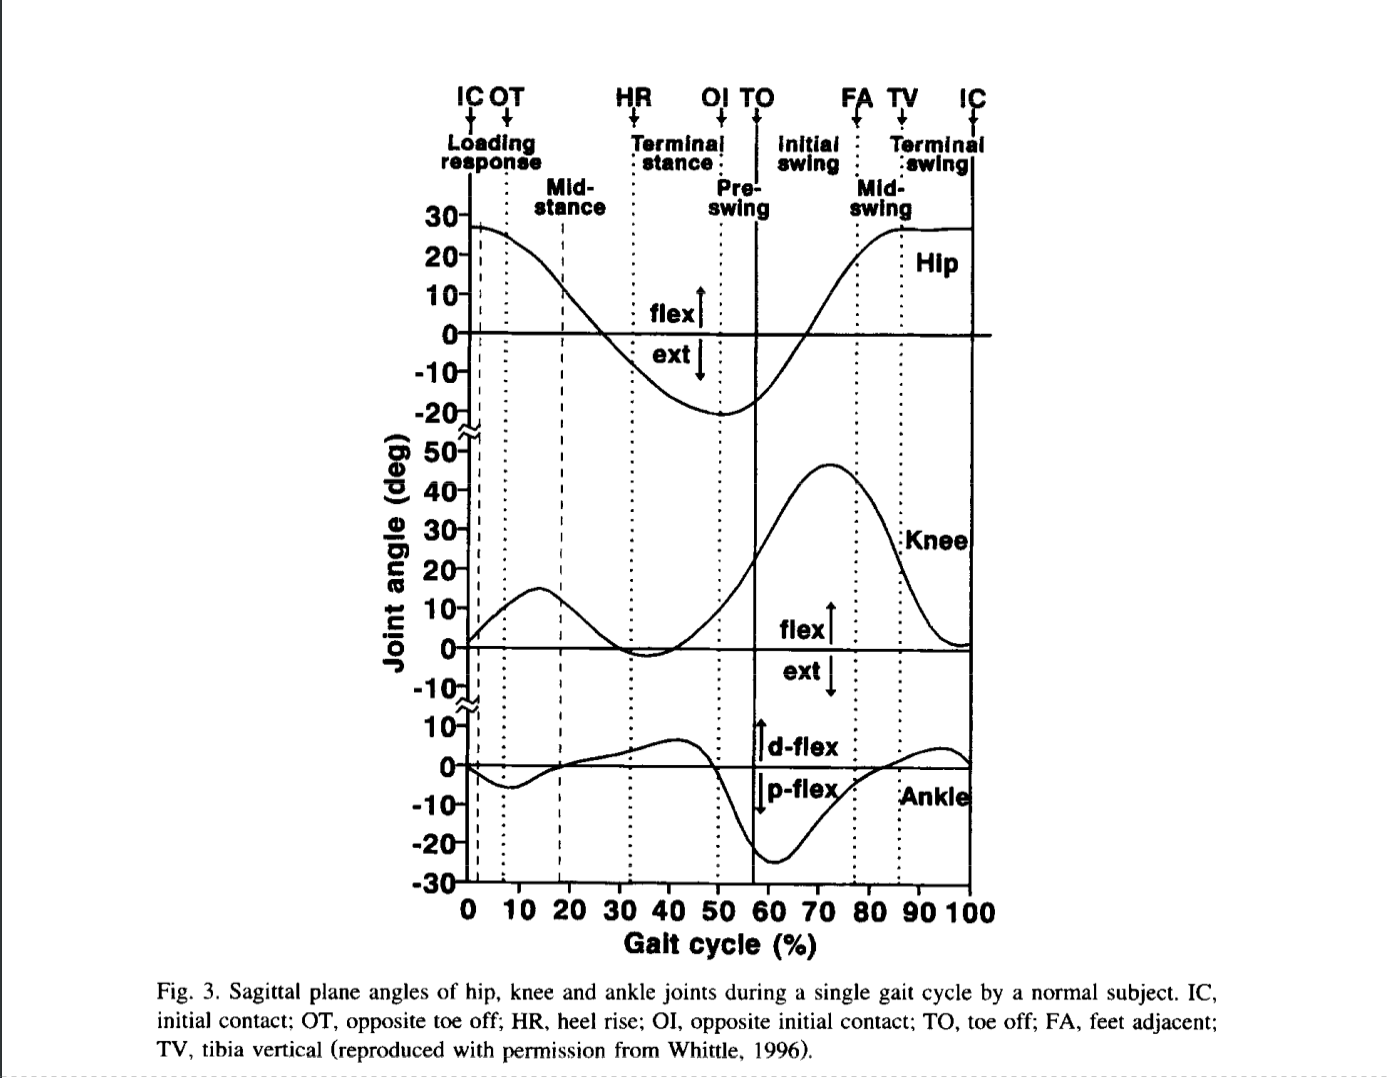
\includegraphics[width=0.7\linewidth]{bilder/Einleitung/gangphasen}
	\caption[Gangphasen]{blabla blabla}
	\label{fig:gangphasen}
\end{figure}


 Durch kinematische und kinetische Beobachtungen lassen sich diese 
\section{Material und Methoden}

\subsection{Proband}
Alle hier dargestellten Daten beziehen sich auf eine männliche Person mit einer Körpergröße l~=~181 cm und einem Gewicht von m~=~75~kg. Neun Gelenke wurden mit Markern versehen, um diese später auszuwerten. Die Gelenke sind: Hals, Schulter, Ellenbogen, Handgelenk, Hüfte, Knie, Knöchel, Ferse und Ballen.

\subsection{Material}
HIER: TABELLE MIT KAMERA, SCHEINWERFERN, LAUFBAND, WAAGE ETC.\\
DANN NUR NOCH BILDER ZEIGEN FÜR DEN AUFBAU\\
AUSRICHTUNG DER KAMERA GENERELL ERKLÄREN
\subsubsection{Laufband}
Der Aufbau besteht aus einem mercury 4.0 Laufband (h/p/cosmos sports \& medical GmbH, Nussdorf-Traunstein, Germany), einer Samsung VP-HMX20C Videokamera (Samsung AG Seoul, Südkorea) und zwei weißen 500W Baustrahlern (MARKE???). Abbildung~\ref{fig:laufbnd_stp} (nicht maßstäblich) zeigt den Aufbau mit der Kamera XX~m vom Laufband entfernt. Die Bildebene ist parallel zur langen Kante des Laufbandes ausgerichtet.

\begin{figure}[h!]
	\centering
	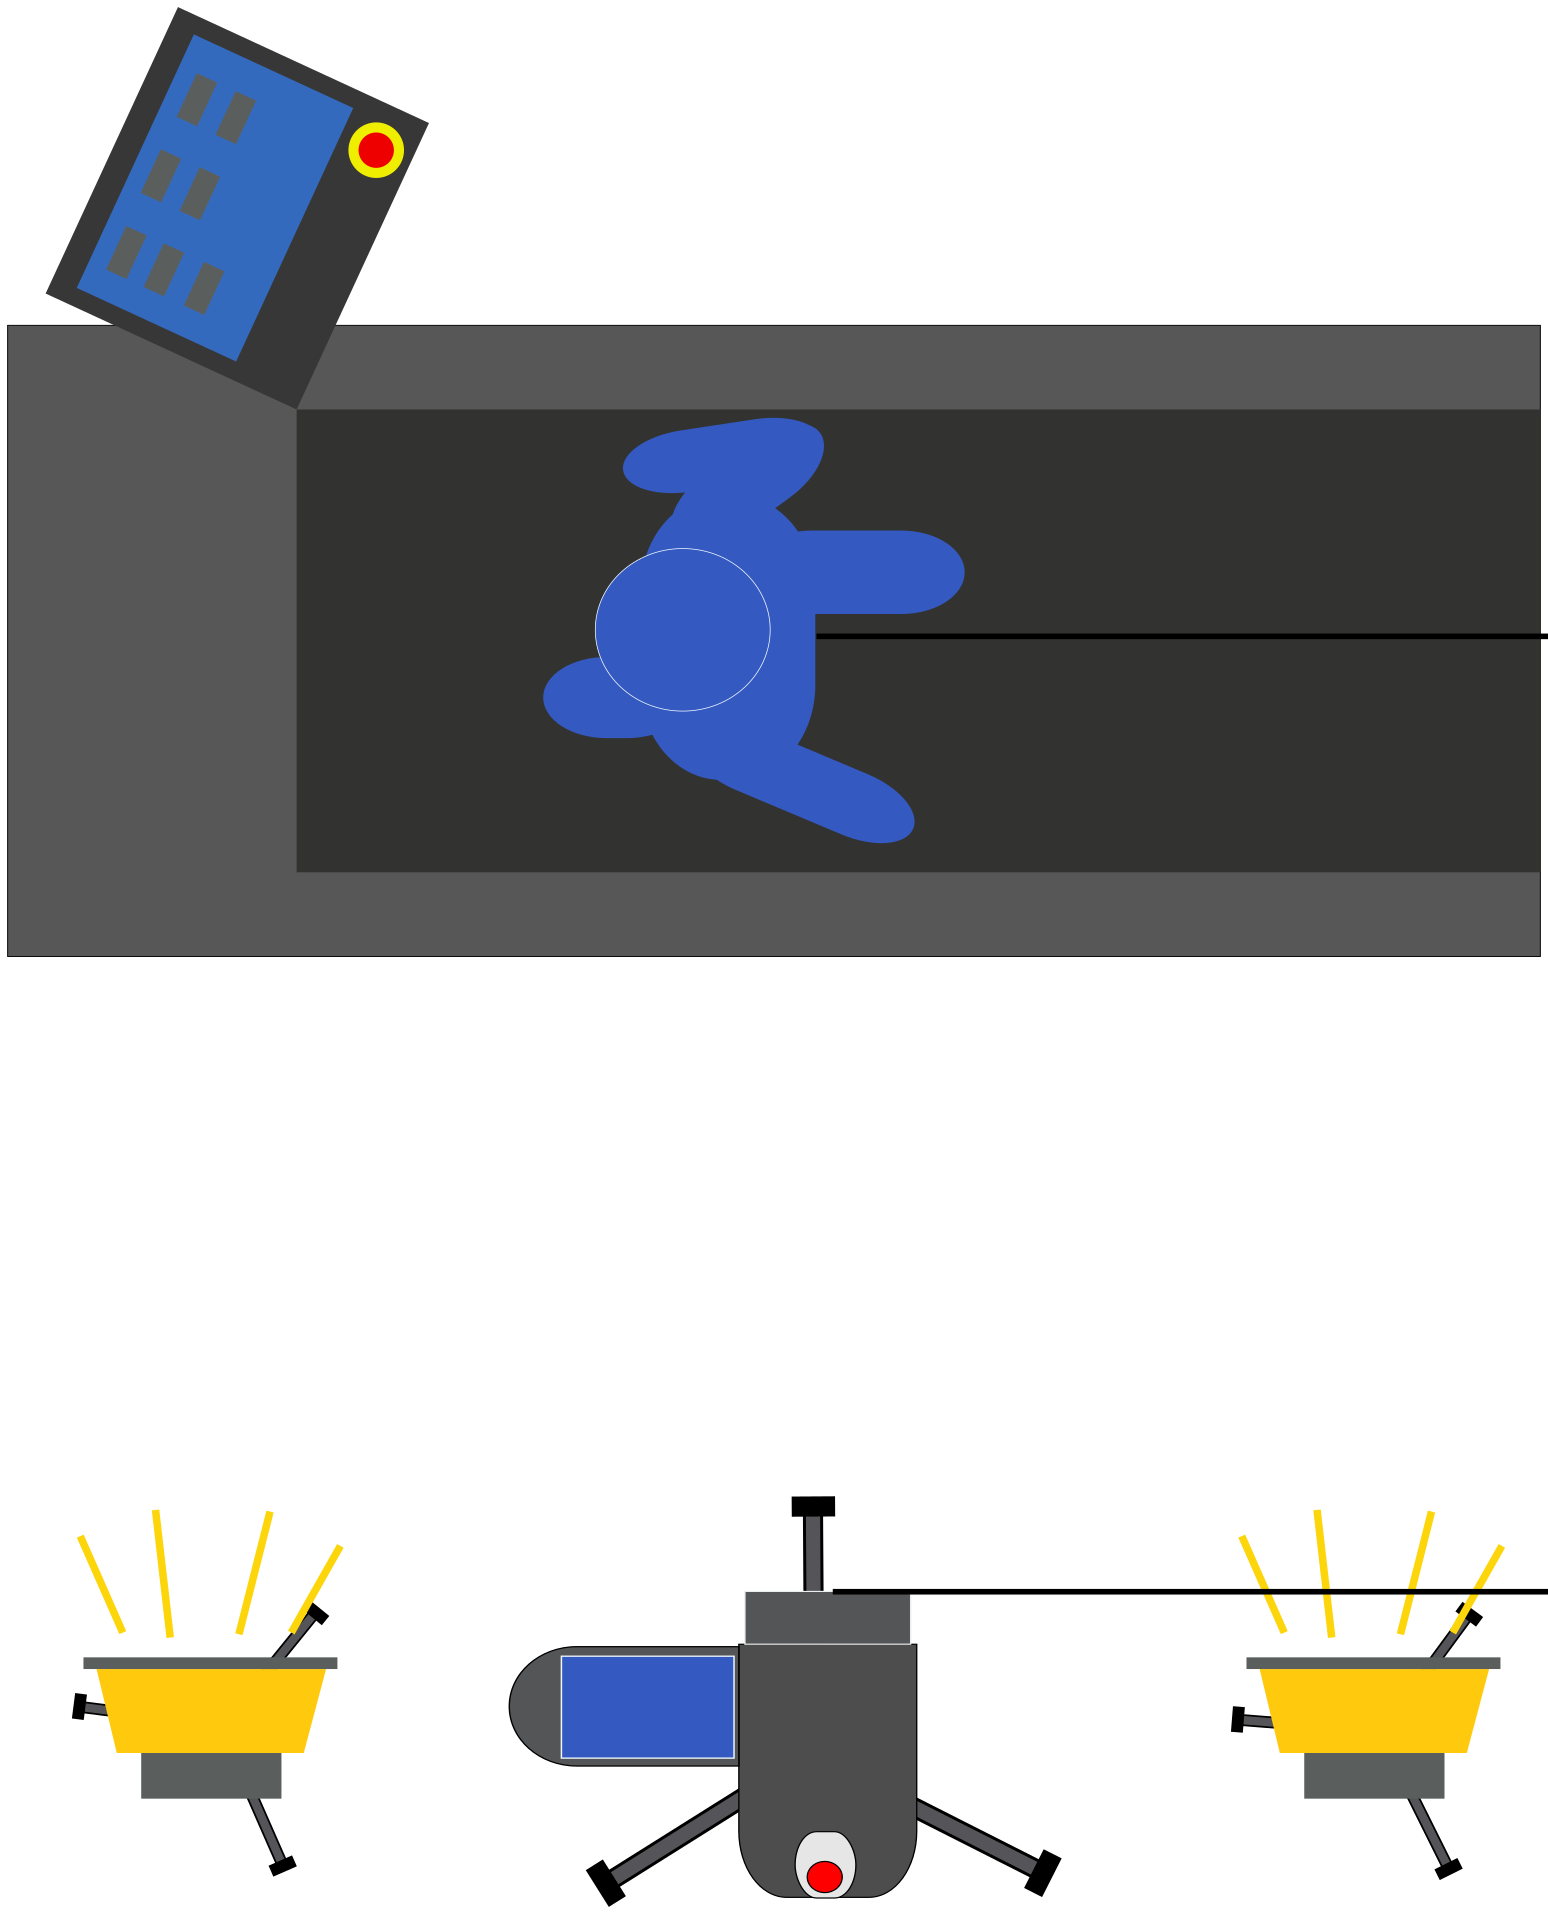
\includegraphics[width=0.5\linewidth]{bilder/mat_met/Laufband_setup}
	\caption[Aufbau Laufband Versuch]{Aufbau des Laufband-Versuches mit Laufband LB, Kamera K und Scheinwerfern SW Abstand zur Kamera $A_{Kam}~=~5~m$ }
	\label{fig:laufbnd_stp}
\end{figure}

\subsubsection{Laufstrecke}
Dieselbe Videokamera und Baustrahler wie bei dem Laufband-Versuchen werden verwendet. Der Proband läuft in diesem Experiment über einen Laufstrecke (Eigenbau Hochschule Bremen, Deutschland). In den Steg ist ein Quarzkristall-3-Komponenten-Dynanometer Typ 9257B (Kistler Gruppe Winterthur, Schweiz) zum Messen der Kräfte eingebaut, welches im Folgenden als Waage bezeichnet wird. Die Waage ist über einen Mehrkanal-Ladungsverstärker Typ 5070A (Kistler) mit einem Computer verbunden. Abbildung~\ref{fig:laufstg_stp} (nicht maßstäblich) zeigt den Aufbau mit der Kamera XX~m vom Laufstrecke entfernt. Die Kamera steht zentriert vor der Waage und die Bildebene ist parallel zur langen Kante des Laufstreckees ausgerichtet.

\begin{figure}[h!]
	\centering
	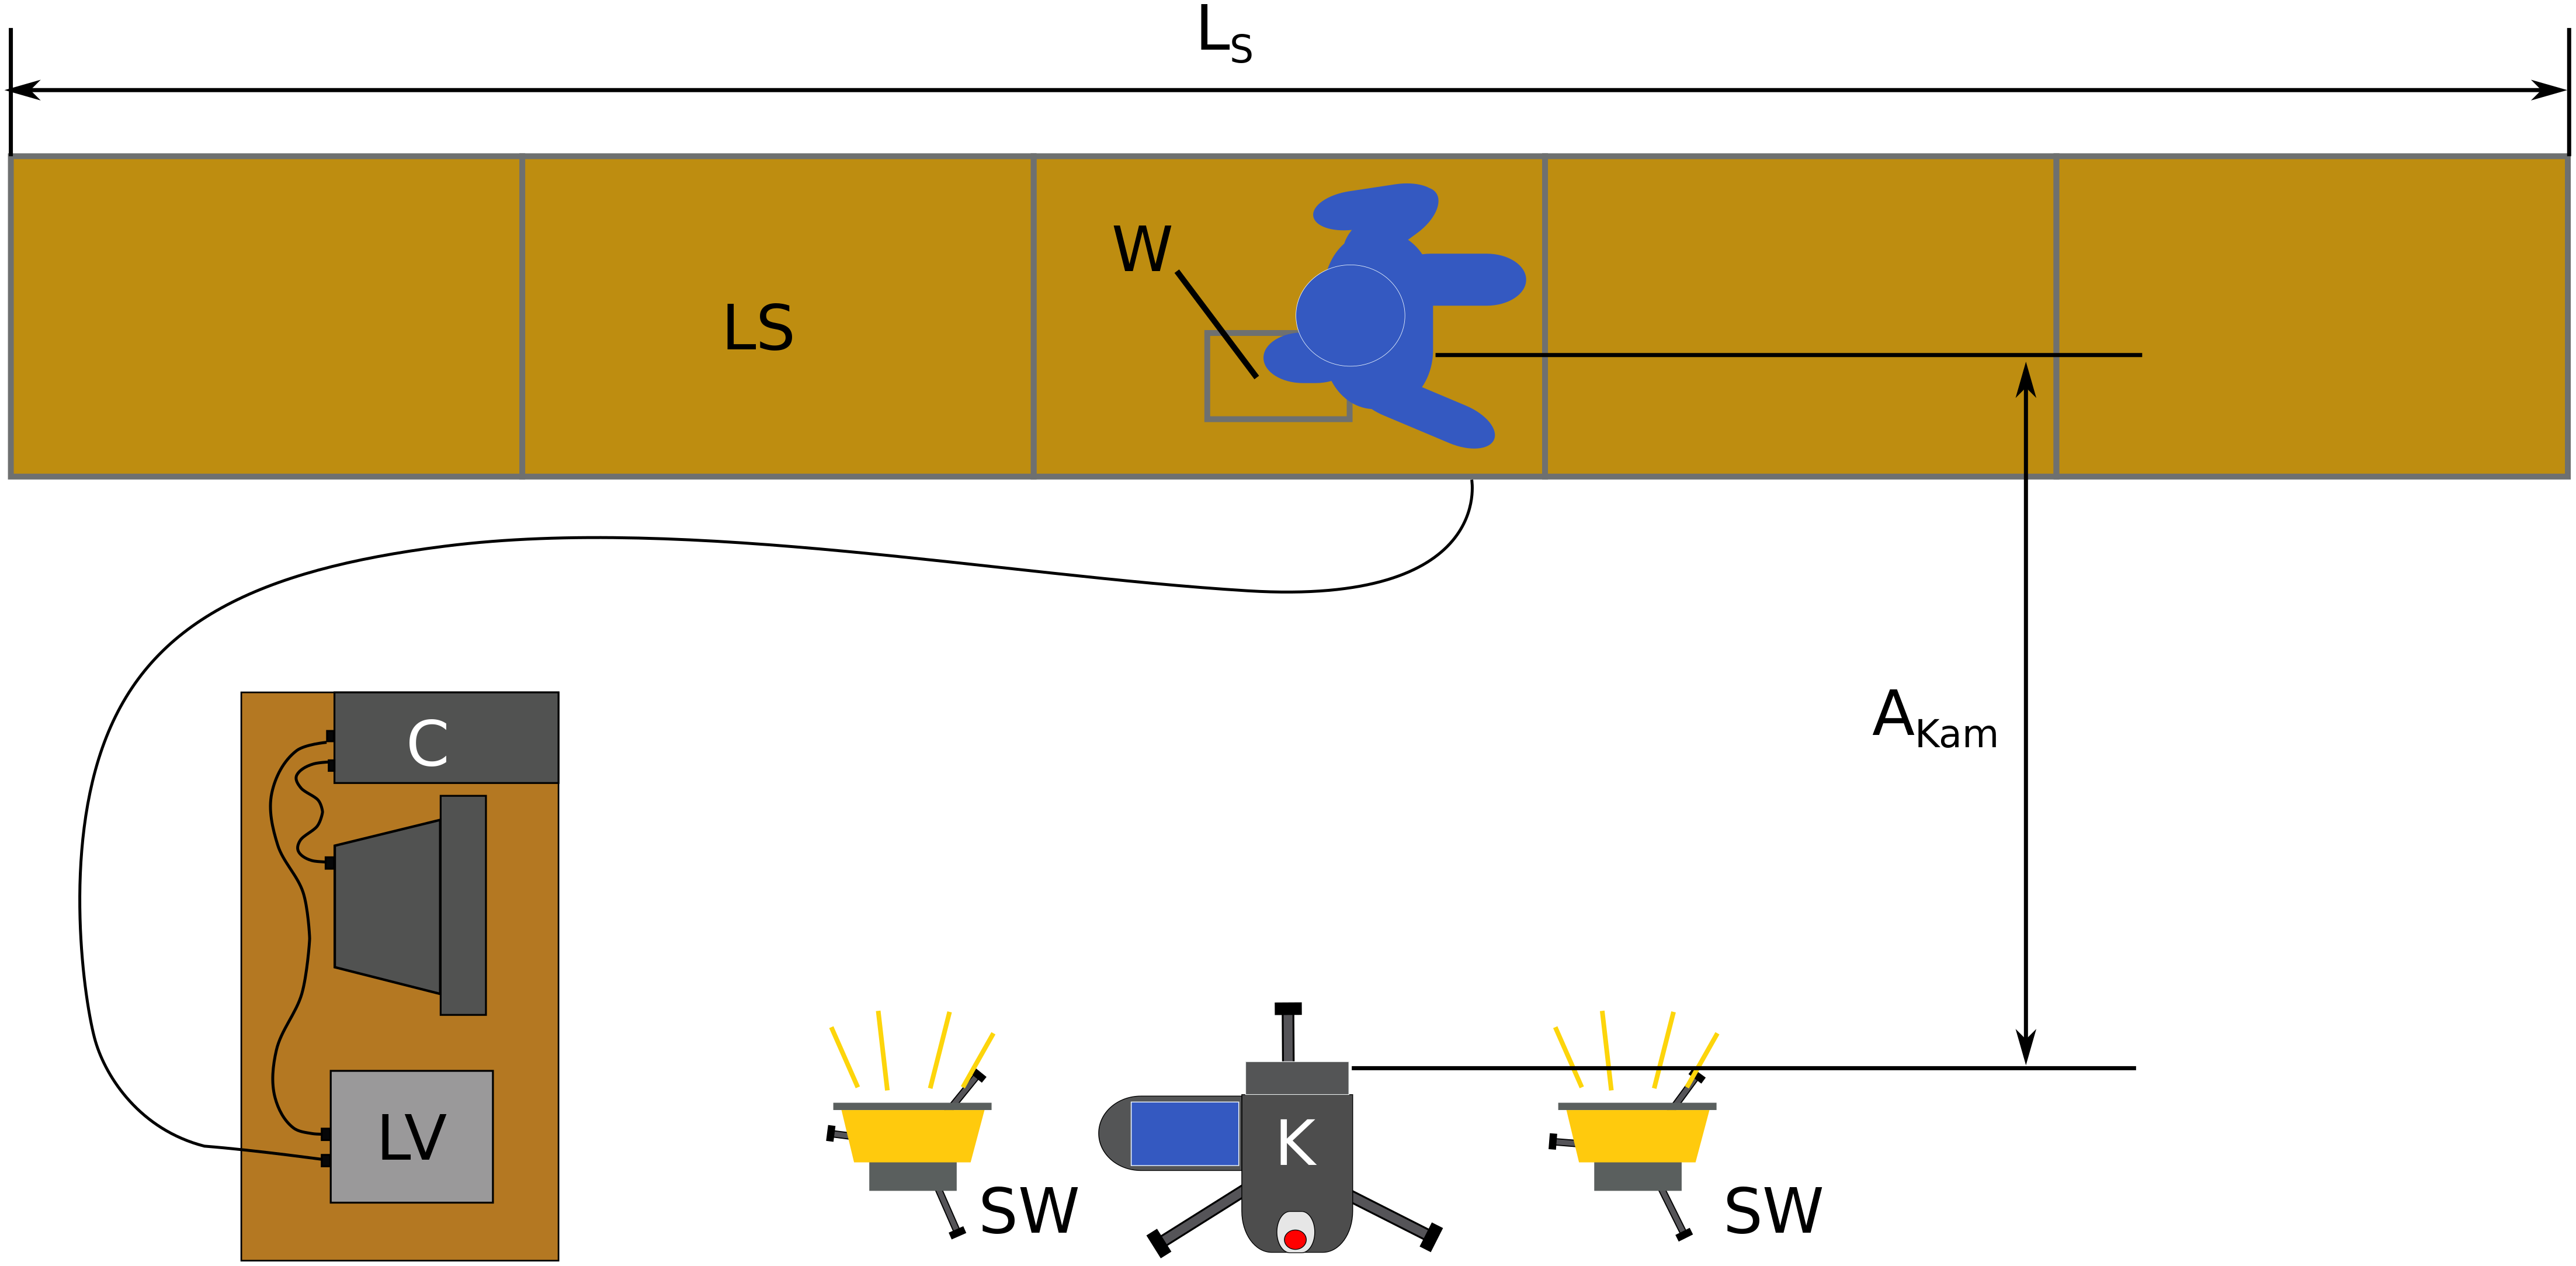
\includegraphics[width=0.7\linewidth]{bilder/mat_met/Laufstrecke_setup}
	\caption[Aufbau Laufstrecke Versuch]{Aufbau des Laufstrecke-Versuches mit Laufstrecke LS, Kamera K, Scheinwerfern SW, Computer C, Waage W und Ladungsverstärker LV. Länge Steg $L_S~=~6~m$ und Abstand zur Kamera $A_{Kam}~=~5~m$}
	\label{fig:laufstg_stp}
\end{figure}

\subsection{Methoden}
\subsubsection{Laufband}
Ausgehend von 1~km/h werden in 1~km/h-Schritten sieben Geschwindigkeiten untesucht. Das Gehen wird subjektiv von 1 (angenehm) bis 10 (unangenehm) bewertet.Je zwei Gangzyklen werden mit einer Bildrate von 50~Hz, einer Belichtung von 1/1000~s und auf 5~m fixierten Fokus aufgenommen.\\
Die Videos werden anschließend mit dem Programm ffmpeg 2.1 (LGP License, ffmpeg.org) in Einzelbilder zerlegt. In ImageJ (National Institutes of Health Bethesda, Maryland) werden mithilfe des Plugins MTrackJ \textbf{CITE(Meijering 20120)} die x- und y-Koordinaten aller Gelenke digitalisiert und im .mdf-Format gespeichert.

\subsubsection{Laufstrecke}
EINSTELLUNGEN LADUNGSVERSTÄRKER???\\
Die Kameraeinstellungen vom Laufbandversuch übernommen finden auch hier Anwendung. Die Digitalisierung der Koordinaten ist wie oben beschrieben durchgeführt worden. Die Waagensignale werden mit 100 Hz und 200~N/V vom Ladungsverstärker an den Computer weitergeleitet. Mit DASYLab werden die Eingangssignale verarbeitet und alle 8 Kanäle im ASCII-Format gespeichert.
Für eine 4-Punkt-Kalibration wird die Waage in alle drei Raumrichtungen mit 0, 1, 3,6 und 7,75~kg belastet. Der Waagendrift wird über 60~s ohne Belastung für jede Raumrichtung ermittelt.\\
Blick geradeaus, um nicht auf den Gang nicht an die Waage anzupassen


\subsection{Datenauswertung mit Scilab}
Aufbau siehe Kirltey et al
Die Rohdaten der X- und Y-Koordinaten und der Waagenmessungen werden für beide Versuche in Scilab ausgewertet. Die verwendetete Vorgehensweise wird daher hier für beide Versuche gebündelt erklärt, um den Arbeitsvorgang deutlich darzustellen.\\\\
X/Y-Koordinaten\\
Glättung\\
Gleitender Mittelwer\\
Plotten\\
Berechnung Winkel\\
Berechnung Beschl.\\
Berechnung Geschw.\\
\\
Die acht Kanäle der Waage werden in X-, Y- und Z-Richtung zusammengefasst. Der Waagendrift wird durch lineare Regression ermittelt und von allen Rohdaten abgezogen.
Für die Kalibration werden die Signale für die vier Gewichte über 1000 Werte gemittelt. Dadurch können den Spannungen tatsächliche Gewichte zugeordnet werden, welche mittels linearer Regression eine Extrapolation für folgende Messungen erlauben. Die 
Waagendaten\\
Kalibration\\
offset in jeder Messung\\
Volt somit in N umgerechnet\\

Inverse Kinematik\\
FELIX WAS HAST DU DA ALLES GEZAUBERT?!?!?


alle rohdaten an scilab gegeben für beide Versuch eund dann asugewertet\\
Gleichungen angeben\\
Daten filtern!\\
\textit{Gleichungen angeben}\\
\textbf{Kalibrierung}\\
- Nullmessung zur Bestimmung des Waagendrifts\\
- Kalibrierungsmessung\\
--> Bestimmung der der Abhängigkeit zwischen Belastungskraft und Messdaten\\
- Reduktion des Waagendrifts\\
- Regressionsgleichung von Messdaten und Belastungskraft bestimmen\\
\textbf{Datenaufnahme}\\
- Kräfte zusammenfassen\\
- Waagendrift aus Rohdaten rausrechnen\\
- Mittels der Kalibrierungsgleichungen die Rohdaten in Kräfte umrechnen\\
\textbf{Skalierung und Synchronisation!!}\\
- Bei der Skalierung wird die Datenrate der Videorate angepasst (hier also nur jeder zweite Datensatz). Gegebenenfalls muss zwischen den Datensätzen interpoliert werden.\\
- Bei der Datensynchronisation findet ein Abgleich des Videomaterials und der Bodenreaktionskräfte statt\\
\textbf{Digitalisierung des Videomaterials}\\
- Skalieren der Videoaufnahme (ACHTUNG! Referenzbild mit Maßstab erforderlich?!?!?)\\
- Tracken von allen Gelenken\\
- Segmentschwerpunkte berechnen (Fuß, Unter- und Oberschenkel)\\
\textbf{Datenberechnung\ KINEMATIK??}\\
- Berechnung von linearen Geschwindigkeiten und Beschleunigungen\\
- Berechnung von Winkelgeschwindigkeiten und Winkelbeschleunigungen\\
\textbf{Datenfilterung (gleitender Mittelwert)}\\
- ACHTUNG! Je nach Anzahl von Stützstellen und Iterationen müssen Bilder vor und nach dem Schrittzyklus in die Digitalisierung einbezogen werden. z.B. 3 Stützstellen und eine Iteration benötigt 1 Bild vorher und ein Bild nachher, um i-1 und n+1 zu berücksichtigen.\\
\textbf{Kinetische Berechnungen (Wagenzentrum rausrechnen?)}\\
Auf der Grundlage von David A. Winter werden:\\
- Kräfte und Momente in den Gelenken berechnet\\
- Berechnung mittels inverser Dynamik\\
\section{Ergebnisse}
\subsection{Laufbandversuch}
Die beste Übereinstimmung für Periodendauer und Frequenz werden für inverses Pendel und Schwerkraftpendel bei 2~km~h$^{-1}$ erreicht. Dabei wird die Periodendauer durch das inverse Pendel unterschätzt (-2,9~\%) und durch das Schwerkraftpendel überschätzt (5,1~\%). Die Abweichungen der Frequenz liegen bei 3,0~\% für inverses Pendel und -4,8~\% für das Schwerkraftpendel. Die geringste Anstrengung wurde bei einer Geschwindigkeit von 3~km~h$^{-1}$ wahrgenommen.

\begin{table}[h!]
\centering
\caption[Ergebnisse Laufbandversuch]{Periodendauer~P und Frequenz~F für einen Doppelschritt bei sieben Geschwindigkeiten. Inverses Pendel (P$_{inv}$, F$_{inv}$) und Schwerkraftpendel (P$_{schw}$, F$_{schw}$) sowie Abweichung in \%.}
\label{tab:Erg_Pend}
\begin{tabular}{c c c c c c c c c c c}
\toprule
Geschw. & Wertung & $P_{inv}$ & Abw. & $F_{inv}$ & Abw. & $P_{schw}$ & Abw. & $F_{schw}$ & Abw. & Schritt-\\
$[km~h^{-1}]$  & [1-10] & [T] & $[\%]$ & [Hz] & $[\%]$ &  [T] & $[\%]$ & [Hz] & $[\%]$ & länge [m]\\
\midrule
Pendel	&---& 1,36 	& ---	& 0,74 	& ---	& 1,90	&---	& 0,52&	---		& ---	\\
1 		& 8	& 1.68 	& 23,6	& 0,60 	&  -19,1& 4,16	& 118,6	& 0,24&	-54,3	& 0,51	\\
2 		& 5 & 1.32 	& -2,9	& 0,76 	&  3,0	& 2,00	& 5,1 	& 0,5 &	-4,8	& 0,54	\\
3 		& 1 & 1.16 	& -14,7	& 0,86 	& 17,2	& 1,44	& -24,3	& 0,69&	32,2	& 0,65	\\
4 		& 3 & 1,00	& -26,4	& 1,00 	& 35,9	& 1,28	& -32,7	& 0,78&	48,7	& 0,73	\\
5 		& 3 & 0.92 	& -32,3	& 1,09 	& 47,7	& 1,12	& -41,2	& 0,89&	69,9	& 0,79	\\
6 		& 5 & 0.88 	& -35,3	& 1,14 	& 54,5	& 1,04	& -45,4	& 0,96&	83,0	& 0,86	\\
7 		& 10& 0.84 	& -38,2	& 1,19 	& 61,8	& 0,92	& -51,7	& 1,09&	106,7	& 0,9	\\
\bottomrule
\end{tabular}
\end{table}

\subsection{Laufstreckenversuch}
Der Vergleich der Bodenreaktionskräfte bei 2, 5 und 7~km~h$^{-1}$ zeigt mit steigender Geschwindigkeit ein Ansteigen der Kraftmaxima und Sinken der -minima bei kürzeren Standphasen (s.~\autoref{fig:res_Kraefte}). Alle drei Kurven zeigen einen kurzen Einbruch des Anstiegs vor dem ersten Maximum. Für 2~km~h$^{-1}$ liegt dieses Maximum bei 93\% des Körpergewichts. Bis auf ein Minimum kurz nach dem Maximum bleibt die Belastung nahezu konstant bis zum Abfallen der Kurve. Für 5~km~h$^{-1}$ liegt das erste Maximum bei 103\% des Körpergewichts, sinkt auf 70\% ab und stiegt erneut auf 109\% an. Für 7~km~h$^{-1}$ liegt das erste Maximum bei 125\%, das Minimum bei 59\% und das zweite Maximum bei 101\%.\\

\begin{figure}[h!]
	\centering
	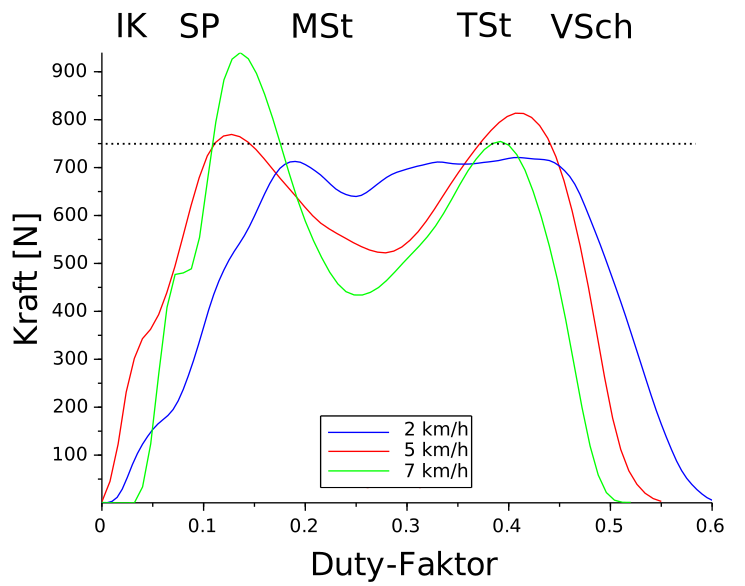
\includegraphics[width=0.7\linewidth]{bilder/Ergebnisse/BRK}
	\caption[Bodenreaktionskräfte]{Vergleich der Bodenreaktionskräfte auf der Laufstrecke bei 2, 5 und 7~km~h$^{-1}$. Gestrichelte Linie stellt das Körpergewicht dar. Standphasen: Initialer Kontakt IK, Stoßdämpfungsphase SP, mittlere und terminale Standphase MSt bzw. TSt sowie Vorschwungphase VSch}
	\label{fig:res_Kraefte}
\end{figure}

Die Kräfte in X-Richtung zeigen in allen Gelenken in der initialen Kontaktphase kurz Werte in Laufrichtung auf, welche mit der Stoßdämpfungsphase entgegen der Laufrichtung wirken. Während der mittleren Standphase wirkt die Kraft wieder in Laufrichtung mit einem Maximum zu Beginn der terminalen Standphase. Der Verlauf der Kräfte in Y-Richtung spiegelt den Verlauf der Bodenreaktionskräfte wieder, jedoch wirkt die Kraft hier in entgegengesetzte Richtung. Der Verlauf der Momente ändert sich erheblich von Gelenk zu Gelenk. Während das Moment im Knöchel während des initialen Kontakts fast bei Null ist, wird es mit Beginn der Stoßdämpfungsphase positiv und bleibt relativ konstant bis zum Ende der terminalen Standphase. In der Vorschwungphase ist es auf Null abgesunken. Im Knie werden wesentlich kleinere Momente er-reicht, welche um Null schwanken. Das Maximum trifft mit dem Beginn der Stoßdämpfungsphase zusammen, sinkt dann während der mittleren Standphase auf Null und wird leicht negativ mit der terminalen Standphase. Der Verlauf des Momentes in der Hüfte ähnelt dem im Knie, ist jedoch deutlich stärker ausgeprägt und zeigt in der Stoßdämpfungsphase starkes Rauschen.\\
\begin{figure}[h!]
	\centering
	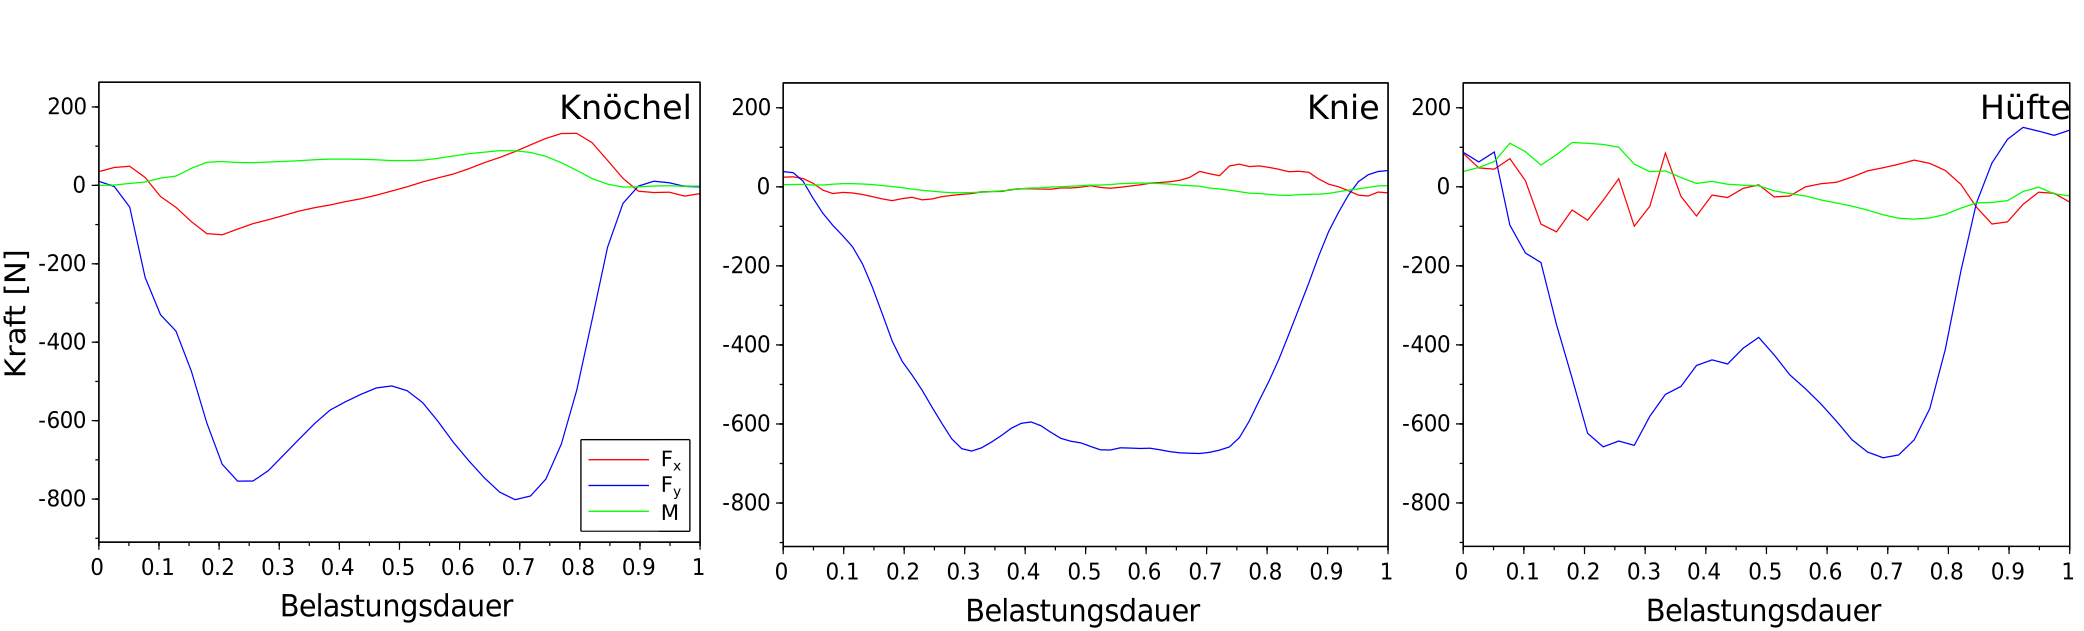
\includegraphics[width=\linewidth]{bilder/Ergebnisse/ang_inv_kin}
	\caption{Kräfte und Momente bei 5~km~h$^{-1}$ in Knöchel-, Knie- und Hüftgelenk}
	\label{fig:ang_inv_kin}
\end{figure}

Wie im vorigen Kapitel sei hier das Knie im Detail mit Fokus auf das Moment dargestellt.
Während das Moment im Knie bei 2~km~h$^{-1}$ nahezu Null ist, ausgenommen zweier kleiner Maxima bei Beginn und Ende des Plateaus der Y-Kraft, zeigt das Moment bei 5~km~h$^{-1}$ deutliche Ausschläge. Während der initialen Kontaktphase und Stoßdämpfungsphase ist das Moment positiv, während es über die mittlere Standphase nahezu Null ist und in der terminalen Standphase einen deutlich negativen Ausschlag hat. Bei 7~km~h$^{-1}$ steigt der positive Ausschlag in der Stoßdämpfungsphase steigt stark an. Das Moment bleibt hier bis kurz vor der terminalen Standphase positiv und hat nur ein sehr geringes negatives Moment in der terminalen Standphase.\\
\begin{figure}[h!]
	\centering
	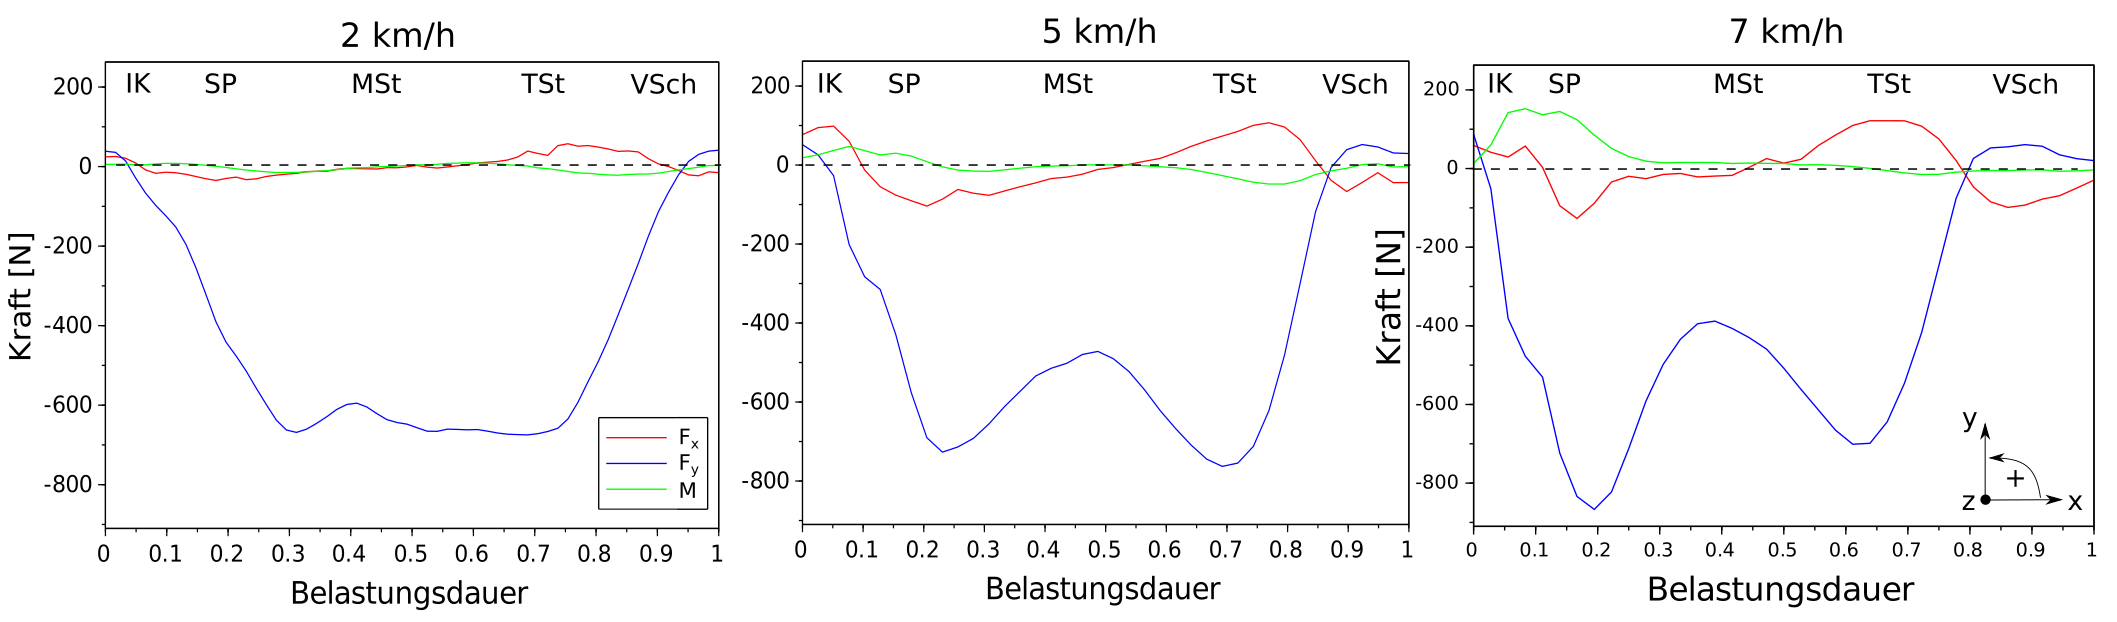
\includegraphics[width=\linewidth]{bilder/Ergebnisse/comp_knee_mom}
	\caption{Kräfte und Momente im Knie-Gelenk bei 2, 5 und 7~km~h$^{-1}$. Standphasen: Initialer Kontakt IK, Stoßdämpfungsphase SP, mittlere und terminale Standphase MSt bzw. TSt sowie Vorschwungphase VSch}
	\label{fig:comp_knee_mom}
\end{figure}

\subsection{Vergleich Laufband und Laufstrecke}
Die auf der Laufstrecke erreichten Geschwindigkeiten entsprechen 2,1~km~h$^{-1}$ (langsam), 4,9~km~h$^{-1}$ (angenehm) und 6,7~km~h$^{-1}$ (schnell) und werden auf ganzzahlige Geschwindigkeiten gerundet.\\
Bei 2~km~h$^{-1}$ ist kein klares Vor- und Zurückschwingen erkennbar und die Hand wird deutlich vor der Körperachse (x~=~0) geführt. Eine deutlichere Schwungbewegung wird bei 5~km~h$^{-1}$ sichtbar. Die X-Amplitude ist auf dem Laufband größer als auf der Laufstrecke. Während die Laufband-Trajektorie vorne abgeflacht ist, beschreibt die Laufstrecken-Trajektorie eine acht. Bei 7~km~h$^{-1}$ steigt die X-Amplitude für beide Versuche weiter an. Beide Trajektorien sind nun flach und weisen in entgegengesetzte Richtungen weisende Krümmungen auf. Der Armschwung findet für Laufband und -strecke vor und hinter der Körperachse statt.\\
Bei allen drei Geschwindigkeiten ist die Körperachse auf dem Laufband mehr nach vorne geneigt als auf der Laufstrecke, bis auf ein Minimum bei 2~km~h$^{-1}$. Während bei 2~km~h$^{-1}$ kein deutliches Schwanken des Winkels der Körperachse um einen Mittelwert zu erkennen ist, kann diese bei 5 und 7~km~h$^{-1}$ deutlich beobachtet werden. Mit dem Wechsel von 5 zu 7~km~h$^{-1}$ verlagert sich der Mittelwert auf dem Laufband von 0$^{\circ}$ zu 2$^{\circ}$, während der Mittelwert für die Laufstrecke von -2$^{\circ}$ auf 0$^{\circ}$ erhöht. Der Körper ist daher auf der Laufstrecke generell weiter nach hinten geneigt als auf dem Laufband.\\
Zum weiteren Vergleich sei hier exemplarisch der Verlauf einer der Gelenkwinkel gezeigt. Der Kniewinkelverlauf ist für den Laufbandversuch über den Doppelschritt dargestellt, während für die Laufstrecke der Fokus aufgrund der inversen Kinetik auf die Standphase gelegt wird.\\
Für alle drei Geschwindigkeiten ist der Verlauf des Winkels auf Laufband und Laufstrecke ähnlich. Für die Sub-Phasen der Standphase wird die Veränderung des Kniewinkels mit der Geschwindigkeit betrachtet. Je schneller der Proband geht, desto stärker ist das Knie gestreckt. Dies ist unabhängig vom Versuch erkennbar durch die kleineren Winkel beim initialen Kontakt (s.~Abb.~\ref{fig:comp_knee_angle}). In der Stoßdämpfungsphase wird das Knie mit steigender Geschwindigkeit deutlich stärker flektiert. Die Flexion steigt von 10$^{\circ}$ beträgt bei 2~km~h$^{-1}$ über 20$^{\circ}$ bei 5~km~h$^{-1}$ auf 26$^{\circ}$ bei 7~km~h$^{-1}$. Bei allen Geschwindigkeiten ist in der mittleren Standphase eine Extension von 16$^{\circ}$ auf dem Laufband und 14$^{\circ}$ auf der Laufstrecke zu beobachten. Der maximale Flexionswinkel wird in der Initialen Schwungphase erreicht und steigt von 63$^{\circ}$ bei 2~km~h$^{-1}$ auf ca. 71$^{\circ}$ bei 5 und 7~km~h$^{-1}$.\\ 

\begin{figure}[h!]
	\centering
	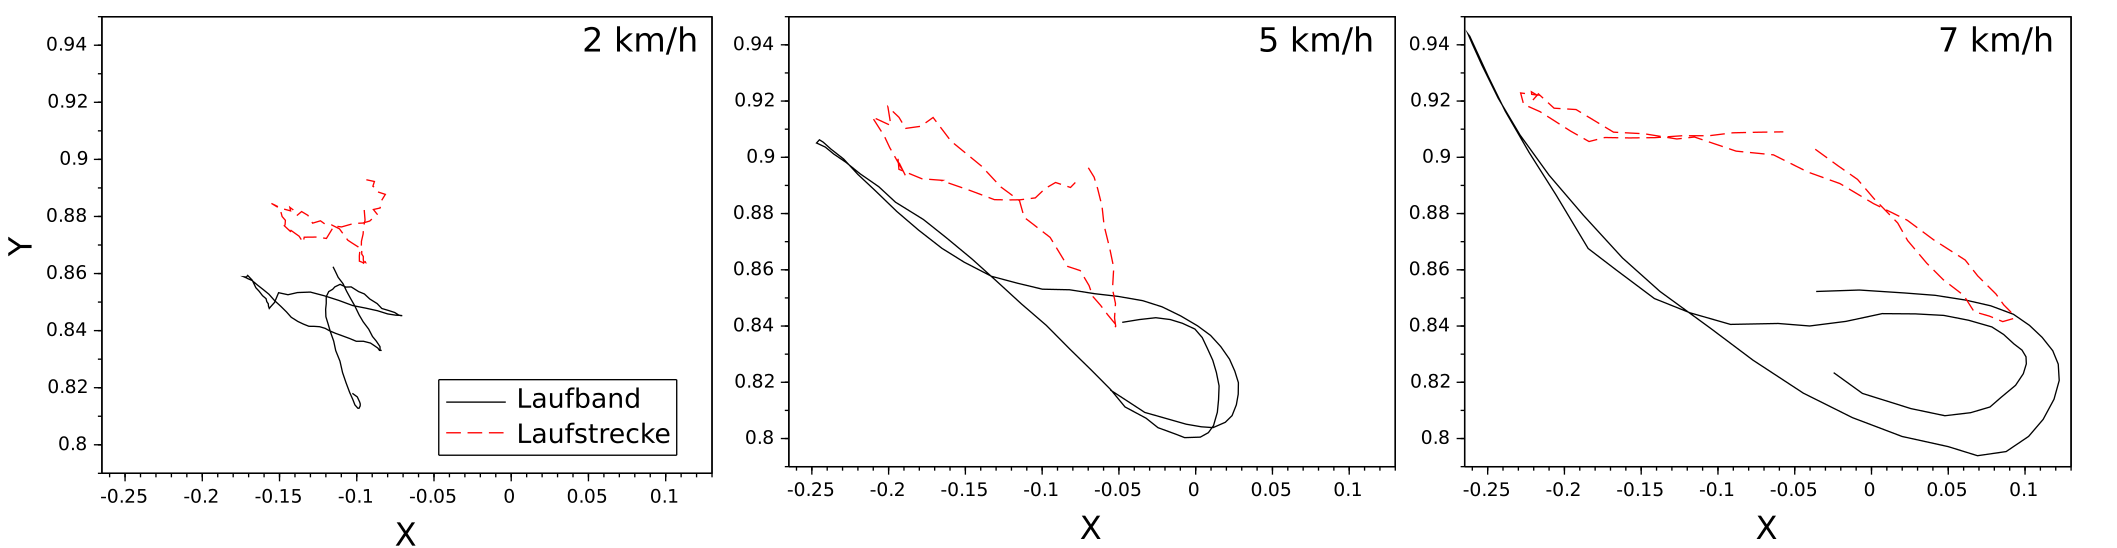
\includegraphics[width=\linewidth]{bilder/Ergebnisse/compare_hand}
	\caption[Handtrajektorien auf dem Laufband und -strecke]{Verlauf der Handtrajektorien auf Laufband und -strecke bei 2, 5 und 7~km~h$^{-1}$. Y-Achse: Höhe über Boden. X-Achse: Auslenkung der Hand. Die Körperachse liegt bei x~=~0.}
	\label{fig:res_compare_hand}
\end{figure}
\begin{figure}[h!]
	\centering
	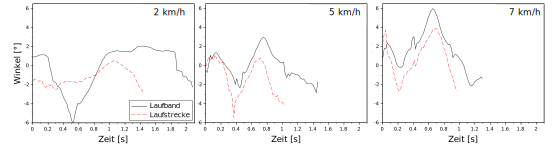
\includegraphics[width=\linewidth]{bilder/Ergebnisse/compare_trunk}
	\caption[Winkelverlauf der Körperachse auf Laufband und -strecke]{Winkelverlauf der Körperachse gegenüber der Horizontalen für Laufband und -strecke bei 2, 5 und 7~km~h$^{-1}$. Aufrechte Körperachse entspricht 0$^{\circ}$, negative Winkel entsprechen zurückgelehnter und positive Winkel vorgebeugter Körperachse}
	\label{fig:res_compare_trunk}
\end{figure}%
\begin{figure}[h!]
	\centering
	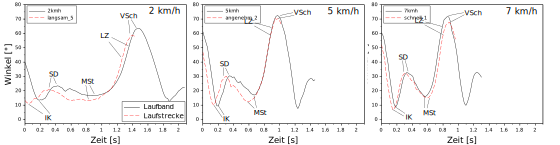
\includegraphics[width=\linewidth]{bilder/Ergebnisse/compare_knee_angle_3_speeds}
	\caption{Verlauf des Kniewinkels über Doppelschritt auf dem Laufband und über Standphase auf der Laufstrecke für 2, 5 und 7~km~h$^{-1}$. Gekennzeichnet sind initaler Kontakt (IK) und Lösen der Zehen (LZ)}
	\label{fig:comp_knee_angle}
\end{figure}

\section{Diskussion}
\subsection{Laufbandversuch}
Am angenehmsten wurde das Gehen bei 3~km~h$^{-1}$ wahrgenommen. Interessanterweise errei-chen das Modell des inversen Pendels sowie das des Schwerpendels die höchste Übereinstimmung bei 2~km~h$^{-1}$. Die Übereinstimmung der beiden Modelle ergibt insofern Sinn, als dass unterschiedliche optimale Geschwindigkeiten für Stand- und Schwungbein nicht zum geringsten Energieverbrauch führen würden. Fehler bei der Ermittlung der Periodendauer können ausgeschlossen werden, da die eingestellte Geschwindigkeit mittels Multiplikation der Doppelschrittdauer und doppelten Schrittlänge (s.~Tab.~\ref{tab:Erg_Pend}) bestätigt werden konnte. 
Ungenauigkeiten durch Verwendung der anthropometrischen Tabelle sind unwahrscheinlich aufgrund der Überlappung der Ergebnisse der beiden Pendelmodelle, wodurch eine genauere Vermessung der Massenverteilung des Beines die Ergebnisse nicht deutlich verändern sollte.\\
Zusätzlich zu der bestehenden Diskrepanz zwischen Messung und Theorie sei hier der Interpretation des Laufstreckenversuches vorweg gegriffen, bei welchem die angenehme Gehgeschwindigkeit bei 5~km~h$^{-1}$ lag und die als langsam und unangenehm empfundene Geschwindigkeit bei 2~km~h$^{-1}$.\\
Die beiden verwendeten Pendelmodelle scheinen hier an ihre Grenzen zu stoßen und die Komplexität des Gehens nicht vollständig zu erfassen. Dies schränkt die Gültigkeit der Annahme eines konstanten Abstandes von Massenschwerpunkt zu Hüfte von \textcite{witte1992mechanische} ein. \textcite{mcmahon1984muscles} konnte zeigen, dass der Kreisbogen des inversen Pendels durch Rotation und seitliches Abkippen des Beckens sowie durch Knieflexion abgeflacht wird. Das Abkippen der Hüfte kann in der Sagittalebene nicht beobachtet werden und bedürfte eine Untersuchung des Gehens in der Frontalebene. Das Gravitationspendel betrachtet das Bein als ein Pendel mit einem Element, wobei sich das Schwungbein als ein Pendel mit drei Elementen exakter beschreiben lässt. Berücksichtigt man diese Aspekte, gewinnt die Modellierung schnell an Komplexität.\\
Es lässt sich zusammenfassen, dass die Modelle des inversen und des Gravitationspendels gute erste Aussagen über das Laufen erlauben, jedoch durch ihre Vereinfachungen auch Fehler eintragen. Es kann mit ihnen die Aussage von \textcite{witte1992mechanische} bestätigt werden, dass das Bein als resonanzschwingunsfähiges System angesehen werden kann. Dass der geringste Arbeitsaufwand für Gehen zwischen 4~km~h$^{-1}$ \parencite{cavagna1976sources} und 4,5~km~h$^{-1}$ \parencite{cavagna2000role} liegt, weicht stark von der als angenehm wahrgenommenen Geschwindigkeit auf dem Laufband ab, deckt sich jedoch gut mit der als angenehm wahrgenom-menen Geschwindigkeit auf der Laufstrecke (5~km~h$^{-1}$). Die starke Abweichung der als angenehm wahrgenommenen Geschwindigkeit kann mit der sehr geringen Zeit zum Einlaufen auf dem Laufband zusammenhängen. Eine längerer Eingewöhnungsphase bei jeder Geschwindigkeit könnte die Wahrnehmung beeinflussen.

\subsection{Laufstreckenversuch}
Zur Überprüfung der Ergebnisse werden die Bodenreaktionskräfte zunächst untersucht. Bei der angenehmen Geschwindigkeit von 5~km~h$^{-1}$ liegen die Maxima bei 103\% und 109\% und das Minimum bei 70\%. Für 5~km~h$^{-1}$ stimmen die Werte gut mit den von \textcite{perry2010gait} ermittelten Durchschnittswerten von je 110\% für die Maxima und 80\% für das Minimum annähernd überein. Es ist jedoch zu erkennen, dass alle prozentualen Werte unter denen von \textcite{perry2010gait} liegen. Dies deckt sich mit der Tatsache, dass das Körpergewicht zu keinem Moment bei 2~km~h$^{-1}$ vollständig vom Standbein getragen wird, wie es eigentlich der Fall sein sollte. Mögliche Ursachen für die zu niedrigen Gewichtswerte scheinen in der Datenaufnahme oder in der Kalibrierung zu liegen, da sich der Gewichtsunterschied auch bei anderen Kommilitonen, welche an anderen Tagen gemessen haben, ausbildete. Eine mögliche Ursache ist in der Kalibrierung zu finden, welche mit 0~kg, 1,5~kg, 3,5~kg und 7,75~kg durchgeführt wurde. Die Toleranz der verwendeten Personenwaage könnte sich bei Gewichten in einer Größenordnung darüber deutlich auswirken. So könnten die 5~kg Abweichung schon durch 0.5~kg Waagentoleranz entstehen. Auch ist zu berücksichtigen, dass während der Kalibrierung der vertikalen Waagenachse die Fußplatte nicht montiert war, welche in Abbildung~\ref{fig:setup_combo}~B dargestellt ist. Diese könnte ebenfalls Einfluss auf die statischen Kräfte durch Gewichtskraft sowie dynamischen Kräfte durch Trägheitskraft genommen haben.\\
Bei allen drei Geschwindigkeiten ist der Übergang zwischen initialem Kontakt und Stoßdämpfungsphase deutlich zu erkennen, gekennzeichnet durch das kurzzeitige Einbrechen des Belastungsanstieges. Diese Stufe ist am Deutlichsten bei 7~km~h$^{-1}$ zu erkennen, wo es zu einem klar abgegrenzten Plateau kommt. Dieses Plateau kommt durch die Flexion des Knies zustande (s.~Abb.~\ref{fig:comp_knee_angle}) und dient dem Abfangen der Belastung bei Bodenkontakt \parencite{perry2010gait}. Da mit steigender Geschwindigkeit der dynamische Anteil der Belastung immer höher wird, steigen auch die Maximalbelastungen in der Stoßdämpfungsphase. Diese Maxima wiederum korrelieren deutlich mit der maximalen Knieflexion, was sich mit den Ergebnissen von \textcite{kirtley1985influence} deckt. Der Duty-Faktor von 0.55 bei 7~km~h$^{-1}$ zeigt hier, dass der Proband sich kurz vor dem Übergang zwischen Gehen und Laufen befindet.\\
Die Momente im Knie unterstützen diese Ergebnisse. Der positive Momentverlauf während der Stoßdämpfungsphase und das negative Maximum in der terminalen Standphase decken sich mit den Daten von \textcite{perry2010gait}. Während der Stoßdämpfungsphase kommt es zu einem positiven Moment im Knie, welches zu einer Flexion führt, wie im Verlauf des Kniewinkels deutlich zu erkennen. Zum Ende der Standphase tritt ein negatives Moment auf, was eine Extension bewirken würde. Trotz des negativen Moments kommt es zu einer noch stärkeren Flexion als in der Stoßdämpfungsphase. Dies zeigt, dass die inverse Kinetik nicht die von den Muskeln aufgebrachten Kräfte berücksichtigt und daher die Bewegung nicht ausschließlich erklären kann.\\
\textcite{perry2010gait} beschreiben zusätzlich ein weiteres positives Moment, welches die Extension des Knies in der Schwungphase einleitet. Dieses konnte nicht beobachtet werden, da mit dem Lösen des Fußes vom Boden keine Bodenreaktionskräfte mehr aufgenommen wurden.\\
Interessant ist hierbei die Entwicklung des Moments im Knie über die drei Geschwindigkeiten unter Berücksichtigung der Knieflexion (s.~Abb.~\ref{fig:comp_knee_mom}). Betrachtet man das Gehen bei 2~km~h$^{-1}$, so ist nur eine geringe Flexion von 22$^{\circ}$ des Knies zu erkennen. Dieses Ergebnis passt zu dem sehr geringen Moment. Die maximale Flexion in der Stoßdämpfungsphase hängt deutlich mit der Geschwindigkeit zusammen. Interessant ist hier, dass sich der Flexionswinkel von 2 auf 5~km~h$^{-1}$  viel stärker verändert als von 5 auf 7~km~h$^{-1}$, das Moment im Knie jedoch zwischen den ersten beiden Geschwindigkeiten nur gering ansteigt und zwischen 5 und 7~km~h$^{-1}$ deutlich größer wird. Es wird vermutet, dass dem positiven Moment bei 5 und 7~km~h$^{-1}$ eine muskuläre Kraft entgegengesetzt wird, welche eine übermäßige Flexion des Knies in der Stoßdämpfungsphase verhindert. Das negative Moment am Ende der terminalen Standphase steigt von 2 zu 5~km~h$^{-1}$ ebenfalls an, ist jedoch bei 7~km~h$^{-1}$ kaum zu erkennen. Obwohl die Knieflexion bei 7~km~h$^{-1}$ mit 72$^{\circ}$ am Stärksten ausgeprägt ist, scheint hierfür am wenigsten Kraft notwendig zu sein. Eine so starke Veränderung des Verlaufs des Moments kann in der Literatur nicht beobachtet werden, was auf die nur einmalige Durchführung des Versuches zurückgeführt wird.\\
Nicht mit der Literatur übereinstimmend ist das Moment im Knöchel, welches durchgängig po-sitiv ist \parencite{eng1995kinetic, lay2006effects, perry2010gait}. Die drei Arbeiten beschreiben im Knöchel ein leicht negatives Moment während der Belastungsantwort aufgrund der Plantarflexion während des Aufsetzens des Fußes. Während der mittleren und terminalen Standphase steigt das Moment dann an und ähnelt den hier gemessenen Werten. Das Maximum des Moments in der terminalen Standphase mit einem Abfallen in der Vorschwungphase kann auch in den Ergebnissen dieser Arbeit beobachtet werden. Aufgrund der einmaligen Durchführung der Versuche wird auf eine Interpretation dieser Abweichung verzichtet, da nicht gesagt werden kann, ob es zum Gangmuster des Probanden gehört.\\
Für das Moment im Hüftgelenk unterscheiden sich die Ergebnisse in der Literatur, jedoch ist bei allen zu Beginn der Standphase ein positives Moment zu beobachten, gefolgt von einem negativen Moment in der terminalen Standphase. Dieses Ergebnis deckt sich mit den hier erhobenen Daten. Auffällig bei den Ergebnissen der X- und Y-Kräfte in der Hüfte sind die starken Aus-schläge am Anfang der Standphase. Diese Schwankungen werden dadurch erklärt, dass zu diesem Zeitraum der Hüftmarker von der Hand verdeckt war und dessen Position abgeschätzt wurde. Hier würde eine größere Anzahl an ausgewerteten Doppelschritten sich sehr stark bemerkbar machen, da solche Artefakte durch die Mittlung stark abgeschwächt würden.


\subsection{Vergleich Laufband und Laufstrecke}
Ein Vergleich der Handtrajektorien bei 2~km~h$^{-1}$ erlaubt keine schlüssige Aussage. Dies kann zum einen an der fehlenden Mittlung über mehrere Doppelschritte liegen, zum anderen daran, dass bei so geringen Geschwindigkeiten die Arme noch keine Ausgleichsbewegungen gegen die Beinbewegung durchführen müssen und die Stabilität des Gehens noch keine dynamische ist, sondern eher ein Balancieren auf der Stelle und damit mehr einer statischen Stabilität gleicht \parencite{barbareschi2015statically}.\\
Bei 5 und 7~km~h$^{-1}$ ist ein deutlicher Unterschied in den Handtrajektorien zwischen den Versuchen zu erkennen. Die stärkere Auslenkung in X- und Y-Richtung bei 5 und 7~km~h$^{-1}$ auf dem Laufband ist interessant unter der Annahme der Arme als passive Masse-Dämpfer nach \textcite{pontzer2009control}. Demnach dienen die Arme der Reduktion der Rotation des Oberkörpers um die Längsachse. Die stärkere Auslenkung auf dem Laufband würde demnach bedeuten, dass hier der Oberkörper stärker zur Rotation neigt, was jedoch durch die stärkere Armbewegung ausgeglichen wird und daher der Energieverbrauch nicht beeinträchtigt sein sollte \parencite{pontzer2009control}. Während andere Arbeitsgruppen deutliche Unterschiede zwischen Laufband und Laufstrecke für Hüftbewegung in der Frontalebene gefunden haben \parencite{alton1998kinematic}, konnten keine derartigen Unterschied für die Armbewegung gefunden werden. Jedoch werden die Ergebnisse dieser Untersuchung wie bei \textcite{alton1998kinematic} auf das ungewohnte Gehen auf dem Laufband zurückgeführt. Das stärkere Schwingen der Arme könnte eine Ausgleichsbewegung für instabiles Gehen auf dem Laufband sein.\\
Die Ergebnisse zu der Körperachse zeigen interessanterweise, dass auf dem Laufband der Körper stärker nach vorne geneigt ist als auf der Laufstrecke. Dies widerspricht den erwarteten Ergebnissen. Aufgrund der tatsächlichen Positionsänderung auf der Laufstrecke wurde erwartet, dass hier die kinetische Energie zur Vorwärtsbewegung aus dem vorgebeugten Oberkörper gewonnen wird. Besonders die Ergebnisse bei 5 und 7~km~h$^{-1}$ zeigen das genaue Gegenteil. Es sei darauf hingewiesen, dass aufgrund der fehlenden Mittlung über mehrere Durchläufe es sich hier auch um Ausreißer handeln könnte. So wurde im Nachhinein festgestellt, dass bei 2~km~h$^{-1}$ auf dem Laufband der Blick nach unten gerichtet war, was großen Einfluss auf den Winkel der Körperachse hat. Dieses Ergebnis wird daher kritisch betrachtet und der stärker nach vorne gebeugte Oberkörper auf dem Laufband auch hier auf die ungewohnte Laufsituation zurückgeführt. Eine mögliche Erklärung ist die beobachtete Wahrnehmung, dass auf dem Laufband die Gefahr bestand, hinten über zu kippen. Dieses Gefühl würde eine unbewusste Haltungsänderung in eine vorgebeugte Lage erklären, welche als sicherer wahrgenommen wird. Für das Gehen auf der Laufstrecke sei noch erwähnt, dass aufgrund der geringen Abmessungen des Raumes nach Passieren des Messbereiches sehr schnell abgebremst werden musste. Dieses Abbremsen könnte ebenfalls mit einem zurückgelehnten Oberkörper in Zusammenhang stehen.

\section{Fazit}
Beide untersuchten Pendel-Modelle erreichten eine relativ gute Übereinstimmung mit der als angenehm wahrgenommenen Geschwindigkeit. Jedoch scheinen die starken Vereinfachungen, wie z.B. das masselose Bein im inversen Pendel-Modell und die fehlende Drei-Segment-Betrachtung des Beines bei dem Gravitationspendel Fehler einzutragen, die die Abweichungen erklären könnten. Die Betrachtung des Beines mit komplexeren Modellen könnte hier eine bessere Abbildung des Systems Bein ermöglichen.\\
Der Vergleich der Armbewegung scheint auf stärkere Momente um die Längsachse auf dem Laufband als auf der Laufstrecke hinzuweisen. Die Hypothese, dass auf der Laufstrecke die tatsächliche Ortsänderung durch ein Vorbeugen des Körpers erreicht wird, konnte nicht bestätigt werden. Interessanterweise ist gerade auf der Laufstrecke der Körper weiter zurückgelehnt. Ungewohntes Gehen auf dem Laufband und ein verfrühtes Abbremsen auf der Laufstrecke wurden hier als einflussreiche Faktoren gesehen. Es wird vermutet, dass eine erneute Durchführung der Versuche mit mehr Eingewöhnung und einer längeren Laufstrecke großen Einfluss auf die Ergebnisse hat und dadurch zu anderen Ergebnissen führen könnte.\\
Die kinetische Untersuchung zeigt große Übereinstimmung mit der Literatur und scheint am Wenigsten von der einmaligen Durchführung der Versuche beeinflusst zu sein. Die inverse Kinetik dagegen zeigt starke Abweichungen in einigen Gelenken für den Momenten-Verlauf. Leider ist eine Interpretation dieser Unterschiede nicht möglich, da nicht sichergestellt werden kann, dass es keine unnatürlichen Ereignisse sind, die zu diesen Ergebnissen führen.\\
Um solche Ausnahmen auszuschließen sollte bei einer Vertiefung der Studien dringend eine statistische Auswertung mehrerer Versuche durchgeführt werden. Diese ermöglicht das Reduzieren von störenden Einflüssen und die Aussagen werden belastbarer. Auch kann das Gangmuster des Probanden dadurch sicherer bestimmt werden und Abweichungen von der Literatur können intensiv analysiert werden. Hier sei die Feststellung von \textcite{groote2008kalman} angeführt, welche feststellten, dass Hautartefakte zu einer nicht korrekten Darstellung der Marker-Trajektorien führen können. Wenn solche Ereignisse keine Regelmäßigkeit aufweisen, ist das Mitteln über mehrere Durchläufe bestens geeignet, um diese Effekte zu reduzieren.

\section{Ausblick}
Die qualitative Untersuchung des menschlichen Ganges eines Probanden erlaubt trotz der einmaligen Durchführung der Versuche interessante Schlüsse. So zeigen die Daten zu den Trajektorien Potential für die Übertragung auf bipedale Robotersysteme. In Kombination mit Lernalgorithmen könnte so das maschinelle Lernen eines Gangmusters enorm beschleunigt werden. Der zeitliche Verlauf der Kräfte und Momente ist essentiell für die Steuerung und Regelung eines solchen Systems. Dies erlaubt eine angepasste Auslegung der Motoren. Hier würden sich weitere Untersuchungen zur muskulären Aktivierung in den verschiedenen Gangphasen anbieten. Diese würden zusammen mit Kräften und Momenten ein Planen der Reaktionen der Steuerung auf verschiedene Lastfälle erlauben. Anstatt ein reagierendes System zu bauen könnte so ein agierendes System geschaffen werden, was nur noch auf Sonderfälle reagiert.\\
Ebenfalls interessant ist das Verständnis des menschlichen Ganges für die Verbesserung von Exoskeletten. \textcite{barbareschi2015statically} beschreiben anschaulich die Verwendung in der Rehabilitation. Hier kann zum Einen durch statische Stabilität die Sicherheit des Patienten zu jedem Zeitpunkt gesichert werden und gleichzeitig durch ein möglichst natürliches Gangmuster des Exoskeletts der Eindruck eines uneingeschränkten Gehens entstehen. Dies ist besonders für das erneute Erlernen des Gehens, wie zum Beispiel nach einem Schlaganfall, von großer Bedeutung \parencite{yin2012emg}. Durch Wiederholung von Bewegungsabläufen kann die neuronale Ansteuerung der Muskulatur wesentlich schneller wieder erlernt werden. Wenn ein Exoskelett diese ermöglichen kann, so besteht die Chance, die Heilungsaussichten zu verbessern sowie die Therapiekosten deutlich senken.

\paragraph*{Fazit}
Inverse kinematics, the estimation of joint kinematics based on measured trajectories of skin-mounted markers, is complicated by instrumental errors and soft tissue artefacts \cite{groote2008kalman}\\

Fehlender Statistik macht es schwer, Aussagen zu beurteilen, welche von der Literatur abweichen, da hier nicht sichergegangen werden kann, dass es sich um tatsächliches gangmuster oder einen Ausreißer handelt. 

Beide untersuchten Pendel-Modelle erreichten eine relativ gute Übereinstimmung mit der als angenehm wahrgenommenen Geschwindigkeit. Jedoch scheinen die starken Vereinfachungen, wie z.B. das masselose Bein im inversen Pendel Modell und die fehlende Drei-Segment-Betrachtung des Beines bei dem Gravitationspendel Fehler einzutragen, die die Abweichungen erklären könnten. Die Betrachtung des Beines mit kompelexeren Modellen könnte hier eine bessere Abbildung des Systems Bein ermöglichen.\\
Der Vergleich der Armbewegung scheint auf stärkere Momente um die Längsachse auf dem Laufband als auf der Laufstrecke hinzuweisen. Die Hypothese, dass auf der Laufstrecke die tatsächliche Ortsänderung durch ein Vorbeugen des Körpers erreicht wird, konnte nicht bestätigt werden. Interessanterweise ist gerade auf der Laufstrecke der Körper weiter zurückgelehnt. Ungewohntes Gehen auf dem Laufband und ein verfrühtes Abbremsen auf der Laufstrecke wurden hier als einflussreiche Faktoren gesehen. Es wird vermutet, dass eine erneute Durchführung der Versuche mit mehr Eingewöhnung und einer längeren Laufstrecke großen Einfluss auf die Ergebnisse hat und dadurch zu anderen Ergebnissen führen könnte.\\
Die kinetische Untersuchung zeigt große Übereinstimmung mit der Literatur und scheint am wenigsten von der einmaligen Durchführung der Versuche beeinflusst zu sein. Die inverse Kinetik dagegen zeigt starke Abweichungen in einigen Gelenken für den Momenten-Verlauf. Leider ist eine Interpretation dieser Unterschiede nicht möglich, da nicht sichergestellt werden kann, dass es keine unnatürlichen Ereignisse sind, die zu diesen Ergebnissen führen.

\paragraph*{Ausblick}
Die qualitative Untersuchung des menschlichen Ganges eines Probanden erlaubt trotz der einmaligen Durchführung der Versuche interessante Schlüsse. So zeigen die Daten zu den Trajektorien Potential für die Übertragung auf bipedale Robotersysteme. In Kombination mit Lernalgorithmen könnte so das maschinelle Lernen eines Gangmusters enorm beschleunigt werden. Der zeitlich Verlauf der Kräfte und Momente ist essentiell für die Steuerung und Regelung eines solchen Systems. Dies erlaubt eine angepasste Auslegung der Motoren. Hier würden sich weitere Untersuchungen zu muskulären Aktivierung in den verschiedenen Gangphasen anbieten. Diese würden zusammen mit Kräften und Momenten ein Planen des Reaktionen der Steuerung auf verschiedene Lastfälle erlauben. Anstatt ein reagierendes System zu bauen könnte so ein agierendes System geschaffen werden, was nur noch auf Sonderfälle reagiert.\\
Ebenfalls interessant ist das Verständnis des menschlichen Ganges für die Verbesserung von Exoskeletten. \textcite{barbareschi2015statically} beschreiben anschaulich die Verwendung in der Rehabilitation. Hier kann zum Einen durch statische Stabilität die Sicherheit des Patienten zu jedem Zeitpunkt gesichert werden und gleichzeitig durch ein möglichst natürliches Gangmuster des Exoskeletts der Eindruck eines uneingeschränkten Gehens entstehen.



%\begin{spacing}{0.05}
%\thispagestyle{plain}
%\section{Quellenverzeichnis}
%\pagestyle{scrheadings}
%\ohead{Quellenverzeichnis}
%\bibliographystyle{chicago}
%\bibliography{bibliographie}
%\end{spacing}

\section{Literatur}
Das Literaturverzeichnis ist nach folgendem Schema zu gestalten: (siehe Skritp)\\


%%---------------------------------------------------------
%% Anhang, falls erforderlich
%%---------------------------------------------------------
\appendix                %% appendix ist keine Umgebung!

\pagenumbering{roman}
\setcounter{page}{1}
\section*{Anhang}%
\end{document}